\setcounter{section}{0}
\section{CĂN BẬC HAI}
\subsection{Trọng tâm kiến thức}
\begin{tomtat}
\subsubsection{Căn bậc hai}
\begin{boxdn}
	Căn bậc hai của số thực không âm là $a$ là số thực $x$ sao cho $x^2=a$.
\end{boxdn}
	\begin{nx}
	\begin{itemize}
	\item Số âm không có căn bậc hai;
	\item Số $0$ có một căn bậc hai duy nhắt là $0$;
	\item Số dương a có đúng hai căn bậc hai đối nhau là $\sqrt{a}$ (căn bậc hai số học của $a$) và $-\sqrt{a}$.
	\end{itemize}
	\end{nx}
\begin{note}
Tính căn bậc hai của một số $a>0$, chỉ cần tính $\sqrt{a}$. Có thể dễ dàng làm điều này bằng cách sử dụng MTCT.
\end{note}
\begin{note}
	\begin{itemize}
		\item
		Phép toán tìm căn bậc hai số học của số không âm gọi là phép khai căn bậc hai hay phép khai phương (gọi tắt là khai phương)
		\item 
		Với hai số $a$\ $b$ không âm, ta có
		\begin{multicols}{2}
			\begin{itemize}
				\item Nếu $a<b$ thì $\sqrt{a}<\sqrt{b}$;
				\item Nếu $\sqrt{a}<\sqrt{b}$ thì $a<b$.
			\end{itemize}
		\end{multicols}
	\end{itemize}
\end{note}
%---------
\subsubsection{Căn thức bậc hai}
\begin{boxdn}
$\sqrt{A}$ xác định khi $A$ lấy giá trị không âm và ta thường viết là $A\ge 0$. Ta nói $A\ge 0$ là {\color{red}điều kiện xác định} (hay điều kiện có nghĩa của) $\sqrt{A}$.
\end{boxdn}
\begin{note}
 Tương tự như căn bậc hai của một số thực không âm, với $A$ là một biểu thức, ta cũng có:
 \begin{itemize}
 	\item Với $A \geq 0$ ta có $\sqrt{A} \geq 0 ;\left(\sqrt{A}\right)^2=A$;
 \end{itemize}
\end{note}
\end{tomtat}
%%%%%%%%%%%%%%%%%%%
\subsection{Các dạng bài tập}
\begin{dang}{Tìm căn bậc hai của một số}
\end{dang}
%%==========Ví dụ 1
\begin{vd}
	Tính
	\begin{listEX}[4]
	\item $\sqrt{81}$;
	\item $\sqrt{16}$;
	\item $-\sqrt{1,21}$;
	\item $-\sqrt{0{,}01}$;	
	\item $\sqrt{0{,}81}$;
	\item $\sqrt{\dfrac{9}{25}}$;
	\item $\sqrt{\dfrac{4}{25}}$;
	\item $-\sqrt{\dfrac{1}{4}}$;
	\end{listEX}
	\loigiai{
	\begin{listEX}[2]
	\item Vì $9^2=81$ nên $\sqrt{81}=9$.
	\item Vì $4^2=16$ nên $\sqrt{16}=4$.
	\item Vì $1{,}1^{2}=1{,}21$ nên $-\sqrt{1,21}=-1,1$.
	\item Vì $(0{,}1)^2=0{,}01$ nên $-\sqrt{0{,}01}=-0{,}1$.
	\item Vì $0{,}9^2=81$ nên $\sqrt{0{,}81}=0{,}9$.
	\item Vì $\left( \dfrac{3}{5}\right)^2=\dfrac{9}{25}$ nên $\sqrt{\dfrac{9}{25}}=\dfrac{3}{5}$.
	\item Vì $\left(\dfrac{2}{5}\right)^2=\dfrac{4}{25}$ nên $\sqrt{\dfrac{4}{25}}=\dfrac{2}{5}$.
	\item Vì $\left(\dfrac{1}{2}\right)^{2}=\dfrac{1}{4}$ nên $-\sqrt{\dfrac{1}{4}}=-\dfrac{1}{2}$.
	\end{listEX}
	}
\end{vd}
%%==========Ví dụ 2
\begin{vd}
	Tìm căn bậc hai của 
	\begin{listEX}[4]
	\item $121$;
	\item $144$;
	\item $64$;
	\item $\dfrac{9}{16}$;
	\item $0{,}25$;
	\item $\dfrac{4}{9}$;
	\item $1{,}44$;
	\item $\left(-\dfrac{2}{5}\right)^2$.
	\end{listEX}	
	\loigiai{
	\begin{listEX}[1]
	\item Ta có $\sqrt{121}=11$ nên $121$ có căn bậc hai là $11$ và $-11$.	
	\item Ta có $\sqrt{144}=12$ nên $144$ có căn bậc hai là $12$ và $-12$.
	\item Ta có $\sqrt{64}=8$ nên $64$ có căn bậc hai là $8$ và $-8$.
	\item Ta có $\sqrt{\dfrac{9}{16}}=\dfrac{3}{4}$ nên $\dfrac{9}{16}$ có căn bậc hai là $\dfrac{3}{4}$ và $-\dfrac{3}{4}$.
	\item Ta có $\sqrt{0{,}25}=0{,}5$ nên $0{,}25$ có căn bậc hai là $0{,}5$ và $-0{,}5$.
	\item Ta có $\sqrt{\dfrac{4}{9}}=\dfrac{2}{3}$ nên $\dfrac{4}{9}$ có căn bậc hai là $\dfrac{2}{3}$ và $-\dfrac{2}{3}$;
	\item Ta có $\sqrt{1{,}44}=1{,}2$ nên $1{,}44$ có căn bậc hai là $1{,}2$ và $-1{,}2$;
	\item Ta có $\sqrt{\left(-\dfrac{2}{5}\right)^2}=\dfrac{2}{5}$ nên $\left(-\dfrac{2}{5}\right)^2$ có hai căn bậc hai là $\dfrac{2}{5}$ và $-\dfrac{2}{5}$.
	\end{listEX}
	}
\end{vd}
%%==========Ví dụ 3
\begin{vd}
	Tìm căn bậc hai của 
	$$256;\, 0{,}04;\, \dfrac{121}{36};\, 11;\, 1{,}6;\, -0{,}09.$$
	\loigiai{
	\begin{itemize}
	\item Căn bậc hai của $256$ là $\pm 12$;
	\item Căn bậc hai của $0{,}04$ là $\pm 0{,}2$.
	\item Căn bậc hai của $\dfrac{121}{36}$ là $\pm\dfrac{11}{6}$.	
	\item Căn bậc hai của $11$ là $\pm\sqrt{11}$;
	\item Căn bậc hai của $1{,}6$ là $\pm\sqrt{1{,}6}$;
	\item Do$-0{,}09<0$ nên$-0{,}09$ không có căn bậc hai.
	\end{itemize}
	}
\end{vd}
%%==========Ví dụ 4
\begin{vd}%[9D1B1]
	Tính giá trị của biểu thức: $\sqrt{0{,}09}+7\cdot\sqrt{0{,}36}-3\cdot\sqrt{2{,}25}$.
	\loigiai{Ta có: $\sqrt{0{,}09}+7\cdot\sqrt{0{,}36}-3\cdot\sqrt{2{,}25}=0{,}3+7\cdot 0{,}6-3\cdot 1{,}5=0{,}3+4{,}2-4{,}5=0$.}
\end{vd}
%%==========Ví dụ 5
\begin{vd}%[9D1Y1]
	Giá trị của biểu thức sau là số vô tỷ hay hữu tỷ: $\sqrt { \left( \sqrt { 1 \dfrac { 9 } { 16 } } - \sqrt { \dfrac { 9 } { 16 } } \right) \cdot 18 }$?
	\loigiai{Ta có: $\sqrt { \left( \sqrt { 1 \dfrac { 9 } { 16 } } - \sqrt { \dfrac { 9 } { 16 } } \right) \cdot 18 }=\sqrt { \left( \sqrt { \dfrac { 25 } { 16 } } - \sqrt { \dfrac { 9 } { 16 } } \right) \cdot 18 }=\sqrt{\left(\dfrac{5}{4} - \dfrac{3}{4}\right)\cdot 18}=\sqrt{9}= 3$.\\Vậy giá trị của biểu thức đã cho là một số hữu tỷ, hơn nữa còn là một số tự nhiên.}
\end{vd}
%----------------
\begin{dang}{Tìm điều kiện xác định của biểu thức chứa căn. Tính giá trị của biểu thức}
	\begin{enumEX}[\itemCI]{2}
	\item $\sqrt{A}$ xác định khi $A\geq 0$.
	\item $\dfrac{1}{\sqrt{A}}$ xác định khi $A>0$.
	\end{enumEX}
\end{dang}
%%==========Ví dụ 6
\begin{vd}%[9D1B2]
	Tìm điều kiện xác định của mỗi căn thức sau:
	\begin{listEX}[4]
	\item $\sqrt{5 - 2x}$;
	\item $\sqrt{\dfrac{1}{x^2 - 4x + 4}}$;
	\item $\sqrt{25-x^2}$;
	\item $\sqrt{\dfrac{1}{x^2 - 100}}$.
	\end{listEX}
	\loigiai{
	\begin{listEX}
	\item
	Điều kiện xác định của căn thức là $5-2x\geq 0$ hay $x\leq\dfrac{5}{2}$.
	\item
	Điều kiện xác định của căn thức là $(x - 2)^2> 0$ hay $x\neq 2$.
	\item 
	Điều kiện xác định của căn thức là 
	$\begin{aligned}[t]
	&25-x^2\geq 0\\
	&x^2\leq 25\\
	&|x|\leq 5\\
	&-5\leq x\leq 5.
	\end{aligned}$
	\item
	Điều kiện xác định của căn thức là 
	$\begin{aligned}[t]
	&x^2-100>0\\
	&x^2>100\\
	&|x|>10\\
	&x>10\text{ hoặc } x<-10.
	\end{aligned}$
	\end{listEX}
	}
\end{vd}
%%==========Ví dụ 7
\begin{vd}%[9D1K2]
	Có bao nhiêu giá trị nguyên của $x$ để biểu thức $M=\sqrt{x+4}+\sqrt{2-x}$ xác định?
	\loigiai{$M$ xác định khi $\heva{&x+4\geq 0\\&2-x\geq 0}$ hay $\heva{&x\geq -4\\&x\leq 2.}$\\Vì $x\in\mathbb{Z}$ nên $x\in\left\lbrace -4; -3; -2; -1; 0; 1; 2\right\rbrace $.\\
	Vậy có $7$ giá trị nguyên của $x$ để biểu thức $M=\sqrt{x+4}+\sqrt{2-x}$ có nghĩa.
	}
\end{vd}
%%==========Ví dụ 8
\begin{vd}
	Xét căn thức $\sqrt{2 x+1}$.
	\begin{enumerate}
	\item Tìm điều kiện xác định của căn thức.
	\item Tính giá trị của căn thức đã cho tại $x=0$ và $x=4$.
	\end{enumerate}
	\loigiai
	{
	\begin{enumerate}
	\item Điều kiện xác định của căn thức là $2 x+1 \geq 0$ hay $x \geq-\dfrac{1}{2}$.
	\item Tại $x=0$ (thoả mãn điều kiện xác định) căn thức có giá trị là $\sqrt{2 \cdot 0+1}=1$.
	Tại $x=4$ (thoả mãn điểu kiện xác định) căn thức có giá trị là $\sqrt{2 \cdot 4+1}=3$.
	\end{enumerate}	
	}
\end{vd}
%%==========Ví dụ 9
\begin{vd}
	Cho biểu thức $A=\sqrt{5-2x}$.
	\begin{listEX}[1]
	\item Với giá trị nào của $x$ thì biểu thức $A$ xác định?
	\item Tính giá trị của biểu thức $A$ khi $x=-2$ và khi $x=3$.
	\end{listEX}
	\loigiai{
	\begin{listEX}[1]
	\item Biểu thức $A$ xác định khi $5-2x \geq 0$ hay $2x\leq 5$ hay $x \leq \dfrac{5}{2}$.
	\item Khi $x=-2$, ta có $A=\sqrt{5-2 \cdot(-2)}=\sqrt{9}=3$.\\
	Ta thấy $x=3>\dfrac{5}{2}$ nên $A$ không xác định tại $x=3$.
	\end{listEX}}
\end{vd}
%%==========Ví dụ 10
\begin{vd} Với giá trị nào của $x$ thì biểu thức $\mathrm{A}=\sqrt{3x+6}$ xác định? Tính giá trị của $\mathrm{A}$ khi $x=5$ (kết quả làm tròn đến chữ số thập phân thứ hai).
	\loigiai{
	Biểu thức $\mathrm{A}=\sqrt{3x+6}$ xác định	khi $3x+6\geq0$ hay $x\geq-2$.\\
	Với $x=5$ ta có $A=\sqrt{3\cdot 5 +6}=\sqrt{21}\approx4{,}58$.
	}
\end{vd}
%-----------------
\begin{dang}{Bài toán so sánh, bài toán tìm $x$}
	\begin{enumerate}[\itemKN]
	\item 
	Với $a, b\geq 0$, ta có:
	$$ \text{Nếu } a < b \text{ thì } \sqrt{a}<\sqrt{b}.$$
	\item
	Với $a\geq 0$, ta có:
	\begin{enumEX}[\itemCI]{3}
	\item $x^2=a$ khi $x=\pm\sqrt{a}$.
	\item $\sqrt{x}=a$ khi $x=a^2$.
	\item $\sqrt{x}<a$ khi $0\leq x<a^2$.
	\end{enumEX}
	\end{enumerate}
\end{dang}
%%==========Ví dụ 21
\begin{vd}
	Không sử dụng MTCT, hãy so sánh:
	\begin{enumEX}{3}
	\item $\sqrt{3}$ và $\sqrt{5}$;
	\item $3$ với $\sqrt{10}$;
	\item $8$ và $\sqrt{65}$.
	\end{enumEX}
	\loigiai{
	\begin{enumerate}
	\item Ta có $3<5$ nên $\sqrt{3}<\sqrt{5}$.
	\item Ta có $10>9$ nên $\sqrt{10}>\sqrt{9}$ hay $\sqrt{10}>3$.
	\item Ta có $64<65$ nên $\sqrt {64} < \sqrt {65}$ hay $8 < \sqrt { 65 }$.
	\end{enumerate}
	}
\end{vd}
%%==========Ví dụ 22
\begin{vd}%[9D1B1]
	Không sử dụng MTCT, hãy so sánh $\sqrt{15}-1$ và $\sqrt{10}$.
	\loigiai{Ta có $\sqrt{15} - 1 <\sqrt{16} - 1 = 4 - 1 = 3$ và $\sqrt { 10 } > \sqrt { 9 } = 3$ nên $\sqrt { 15 } - 1 < \sqrt { 10 }$.}
\end{vd}
%%==========Ví dụ 23
\begin{vd}%[9D1B1]
	Với $a<0$ thì số nào lớn hơn trong hai số $\sqrt{-a}$ và $\sqrt{-2a}$?
	\loigiai{Ta có $-1>-2$ nên $-a<-2a$ (vì $a<0$). Do đó $\sqrt{-a}<\sqrt{-2a}$.}
\end{vd}
%%==========Ví dụ 24
\begin{vd}%[9D1B1]
	Tìm $x$ biết
	\begin{listEX}[3]
	\item $3x^2 = 0{,}75$;
	\item $2\sqrt{3x}= 12$;
	\item $\dfrac{1}{2}\sqrt{5x}< 10$.
	\end{listEX} 
	\loigiai{
	\begin{listEX}[2]
	\item!
	Ta có $3x^2 = 0{,}75$ suy ra $x^2=0{,}25$. Do đó $x =\pm\sqrt{0{,}25}=\pm 0{,}5$.
	\item
	Điều kiện xác định: $x\geq 0$.\\Ta có
	$\begin{aligned}[t]
	2\sqrt{3x}&= 12\\
	\sqrt{3x}&= 6\\
	3x &= 36\\
	x &= 12 \,(\text{thỏa mãn điều kiện}).
	\end{aligned}$
	 \item 
	 Điều kiện xác định: $x\geq 0$.\\ Ta có 
	 $\begin{aligned}[t]
	 	\dfrac{1}{2}\sqrt{5x}&< 10\\
	 	\sqrt{5x}&< 20\\
	 	5x &< 400\\
	 	x &< 80.
	 \end{aligned}$
	 \\Vậy $0 \leq x < 80$.
	\end{listEX}
	}
\end{vd}
%%==========Ví dụ 25
\begin{vd}
	Tìm $x$, biết
	\begin{enumEX}{4}
	\item $x^2=\dfrac{16}{9}$;
	\item $x^2=4-2\sqrt{3}$;
	\item $(x-1)^2=\dfrac{1}{9}$;
	\item $x^2+1=6-2\sqrt{6}$.
	\end{enumEX}
	\loigiai{
	\begin{enumEX}{2}
	\item 
	$\begin{aligned}[t]
	\text{Ta có } 
	x^2 &= \dfrac{16}{9} \\
	x^2 &= \left(\dfrac{4}{3}\right)^2 \\
	x &=\dfrac{4}{3} \text{ hoặc } x=-\dfrac{4}{3}.
	\end{aligned}$ \\
	Vậy $x\in\left\{-\dfrac{4}{3};\dfrac{4}{3}\right\}.$
	\item 
	$\begin{aligned}[t]
	\text{Ta có } x^2 &= 4-2\sqrt{3} \\
	x^2 &= \left(\sqrt{3}-1\right)^2 \\
	x &= \sqrt{3}-1 \text{ hoặc } x=1-\sqrt{3}.
	\end{aligned}$\\
	Vậy $x\in \left\{\sqrt{3}-1;1-\sqrt{3}\right\}.$
	\item 
	$\begin{aligned}[t]
	\text{Ta có } 
	(x-1)^2 &= \dfrac{1}{9} \\
	(x-1)^2 &= \left(\dfrac{1}{3}\right)^2 \\
	x-1 &=\dfrac{1}{3} \text{ hoặc } x-1=-\dfrac{1}{3} \\
	x &=\dfrac{4}{3} \text{ hoặc } x=\dfrac{2}{3}
	\end{aligned}$ \\
	Vậy $x\in\left\{-\dfrac{4}{3};\dfrac{2}{3}\right\}.$
	\item 
	$\begin{aligned}[t]
	x^2+1&=6-2\sqrt{6} \\
	x^2&=5-2\sqrt{6}\\
	x^2&=(\sqrt{3}-\sqrt{2})^2 \\
	x&=\sqrt{3}-\sqrt{2} \text{ hoặc } x=\sqrt{2}-\sqrt{3}.
	\end{aligned}$ \\
	Vậy $x\in\left\{\sqrt{2}-\sqrt{3};\sqrt{3}-\sqrt{2}\right\}$.
	\end{enumEX}
	}
\end{vd}
%%==========Ví dụ 26
\begin{vd}%[9D1B1]
	Tính tổng các giá trị của $x$ thỏa mãn đẳng thức $\sqrt{x^2 + 25}= 13$.
	\loigiai{
	Ta có 
	$\begin{aligned}[t]
	\sqrt{x^2 + 25}&= 13\\
	x^2 + 25 &= 169\\
	x^2&= 169 - 25\\
	x^2&= 144\\
	x &=\pm 12.
	\end{aligned}$
	\\
	Vậy tổng các giá trị của $x$ thỏa mãn đẳng thức đã cho là $( - 12 ) + 12 = 0$.
	}
\end{vd}

%-----------------
\begin{dang}{Bài toán thực tế}
\end{dang}
%%==========Ví dụ 28
\begin{vd}
	Trong một thí nghiệm, một vật rơi tự do từ độ cao $80\ \mathrm{m}$ so với mặt đất. Biết quãng đường dịch chuyển được của vật đó tính theo đơn vị mét được cho bởi công thức $h=5t^2$ với $t$ là thời gian vật đó rơi, tính theo đơn vị giây ($t>0$). Hỏi sau bao nhiêu lâu kể từ lúc rơi thì vật đó chạm đất?
	\loigiai{
	Khi vật chạm đất thì quãng đường dịch chuyển được của vật đó là $80\ \mathrm{m}$.\\
	Ta có $80=5t^2$ hay $t^2=16$. Do đó $t=\sqrt{16}=4$ hoặc $t=-\sqrt{16}=-4$.\\
	Vì $t>0$ nên $t=4$. Vậy sau $4$ giây kể từ lúc rơi thì vật đó chạm đất.
	}
\end{vd}
%%==========Ví dụ 29
\begin{vd}
	\immini{
	Biết rằng hình $A$ và hình vuông $B$ trong Hình $2$ có diện tích bằng nhau. Tính độ dài cạnh $x$ của hình vuông $B$.
	}
	{
	\begin{tikzpicture}[line join=round,line cap=round,>=stealth,font=\footnotesize,scale=0.8]
	\def\canh{3}
	\coordinate (D) at (0,\canh);
	\coordinate (B) at (\canh,\canh);
	\coordinate (A) at (0,0);
	\coordinate (C) at ($(B)+(A)-(D)$);
	\coordinate (x) at ($(B)!1/3!(D)$);
	\coordinate (y) at ($(C)!2/3!(B)$);
	\coordinate (z) at ($(x)+(y)-(B)$);
	\draw (A)--(D)--(x)--(z)--(y)--(C)--(A);
	\draw [dashed](x)--(B)--(y);
	\foreach \i/\g in {A/60}{\draw[fill=black](\i) circle (1.5pt) ($(\i)+(\g:4mm)$) node[scale=1]{$\i$};}
	\node[below] at ($($(A)+(0,-0.25)$)!0.5!($(C)+(0,-0.25)$)$){$3\mathrm{~cm}$};
	\draw[<->] ($(A)+(0,-0.2)$)--($(C)+(0,-0.2)$);
	\node[left=0.3cm] at ($($(A)$)!0.5!($(D)$)$){$3\mathrm{~cm}$};
	\draw[<->] ($(A)+(-0.2,0)$)--($(D)+(-0.2,0)$);
	\node[above=0.4cm] at ($($(x)+(0,-0.25)$)!0.5!($(B)+(0,-0.25)$)$){$\sqrt{2}\mathrm{~cm}$};
	\draw[<->] ($(x)+(0,0.2)$)--($(B)+(0,0.2)$);
	\node[right=0.2cm] at ($($(B)$)!0.5!($(y)$)$){$\sqrt{2}\mathrm{~cm}$};
	\draw[<->] ($(B)+(0.2,0)$)--($(y)+(0.2,0)$);
	\begin{scope}[shift={(6,0)},rotate=0]
	\def\canh{2.7}
	\coordinate (A) at (0,\canh);
	\coordinate (D) at (\canh,\canh);
	\coordinate (B) at (0,0);
	\coordinate (C) at ($(B)+(D)-(A)$);
	\draw(A)--(B)--(C)--(D)--cycle;
	\foreach \i/\g in {B/60}{\draw[fill=black](\i) circle (1.5pt) ($(\i)+(\g:4mm)$) node[scale=1]{$\i$};}
	\node[below] at ($($(B)+(0,-0.25)$)!0.5!($(C)+(0,-0.25)$)$){$x\mathrm{~cm}$};
	\draw[<->] ($(B)+(0,-0.2)$)--($(C)+(0,-0.2)$);
	\end{scope}
	\end{tikzpicture}
	}\loigiai{
	Diện tích hình A là $3^2-\sqrt{2}^2=7$ cm$^2$.\\
	Theo đề ta có diện tích hình B cũng là $7$ cm$^2$.\\
	Suy ra $x=\sqrt{7}$ cm.
	}
\end{vd}
%%==========Ví dụ 30
\begin{vd}
	Vận dụng Trở lại tình huống mở đầu.\\
	Trong Vật lí, quãng đường $S$ (tính bằng mét) của một vật rơi tự do được cho bởi công thức $S=4{,}9t^2$, trong đó $t$ là thời gian rơi (tính bằng giây). Hỏi sau bao nhiêu giây thì vật sẽ chạm đất nếu được thả rơi tự do từ độ cao $122{,}5$ mét?
	\begin{enumerate}
	\item Viết công thức tính thời gian $t$ (giây) cần thiết để vật rơi được quãng đường $S$ (mét).
	\item Sử dụng công thức tìm được trong câu a, hãy trả lời câu hỏi trong tình huống mở đầu.
	\end{enumerate}
	\loigiai
	{
	\begin{enumerate}
	\item Từ công thức $S=4{,}9t^2\Rightarrow t^2=\dfrac{S}{4{,}9}\Rightarrow t=\sqrt{\dfrac{S}{4{,}9}}$ (vì $t>0$).\\
	\item Vật đang ở độ cao $122{,}5$ rơi chạm đất thì vật đã rơi được quãng đường là $S=122{,}5$ (m).\\
	Thay $S=122{,}5$ m vào phương trình $t=\sqrt{\dfrac{S}{4{,}9}}\Rightarrow t=\sqrt{\dfrac{122{,}5}{4{,}9}}=5$ (s).\\
	Vậy sau $5$ (s) thì vật rơi chạm đất.
	\end{enumerate}	
	}
\end{vd}
%%==========Ví dụ 31
\begin{vd}
	Để lái xe an toàn khi đi qua đoạn đường có dạng cung tròn, người lái cần biết tốc độ tối đa cho phép là bao nhiêu. Vì thế, ở những đoạn đường đó thường có bảng chỉ dẫn cho tốc độ tối đa cho phép của ô tô. Tốc độ tối đa cho phép $v$(m/s) được tính bởi công thức $v=\sqrt{rg\mu}$, trong đó $r$(m) là bán kính của cung đường, $g=9{,}8$m/s$^2$, $\mu=0{,}12$ là hệ số ma sát trượt của đường. Tính tốc độ tối đa cho phép $v$ (m/s) để lái xe an toàn khi đi qua đoạn đường có dạng cung tròn vối bán kính $r=400$ m (làm tròn kết quả đến hàng phần mười).
	\loigiai{
	Ta có công thức:
	\[ v = \sqrt{rg\mu} \]
	Thay: $r = 400$ , $g = 9{,}8$, và $\mu = 0{,}12$, ta có:
	\[ v = \sqrt{400 \cdot 9{,}8 \cdot 0{,}12} \approx 22 \, \text{m/s} \]
	Vậy tốc độ tối đa cho phép là khoảng $22$m/s .
	}
\end{vd}
%%==========Ví dụ 32
\begin{vd}
	Một trạm phát sóng được đặt ở vi trí $B$ cách đường tàu một khoảng $AB=300$ (m). Đầu tàu đang ở vi trí $C$, cách vị trí $A$ một khoảng $AC=x$ (m).
	\immini{\begin{listEX}[1]
	\item Viết biểu thức biểu thi khoảng cách từ trạm phát sóng đến đầu tàu.
	\item Tính khoảng cách trên khi $x=400, x=1000$ (kết quả làm tròn đến hàng đơn vị của mét).
	\end{listEX}}{\begin{tikzpicture}[line join=round,line cap=round,>=stealth,font=\footnotesize,scale=0.8]
	\def\canh{2.7}
	\coordinate (A) at (0,0);
	\coordinate (C) at (0:3);
	\coordinate (B) at (90:2.5);
	\draw[dashed](A)--(B)--(C);
	\foreach \i/\g in {A/-90,B/60,C/-90}{\draw[fill=black](\i) circle (1.5pt) ($(\i)+(\g:4mm)$) node[scale=1]{$\i$};}
	\node[below] at ($($(A)+(0,-0.25)$)!0.5!($(C)+(0,-0.25)$)$){$x\mathrm{~cm}$};
	\node[left] at ($($(A)+(0,-0.25)$)!0.5!($(B)+(0,-0.25)$)$){$300\mathrm{~m}$};
	\node[right=0.3cm] at ($($(B)+(0,-0.25)$)!0.5!($(C)+(0,-0.25)$)$){$?$};
	\draw[dashed,line width=2pt] ($(A)+(180:0.3cm)$)--($(C)+(0:1cm)$);
	\end{tikzpicture}}
	\loigiai{
	\begin{listEX}[1]
	\item Biểu thức biểu thi khoảng cách từ trạm phát sóng đến đầu tàu là $BC=\sqrt{90~000+x^2}$.
	\item Với $x=400$ thì $BC=\sqrt{90~000+400^2}=500$ (m).\\
	Với $x=1000$ thì $BC=\sqrt{90~000-1000^2}\approx1044$ (m).
	\end{listEX}
	}
\end{vd}
%==================
\begin{dang}{Tìm giá trị lớn nhất, nhỏ nhất có chứa căn}
\end{dang}
%%==========Ví dụ 33
\begin{vd}%[9D1K1]
	Tìm giá trị nhỏ nhất của biểu thức
	\begin{enumEX}{2}
	\item $A=5+\sqrt{x^2-3x+9}$;
	\item $B=\sqrt{x^2-7x+5}$;
	\item $C=\sqrt{x^2-7x+6}-25$;
	\item $D=8+\sqrt{x^2+3x-4}$.
	\end{enumEX}
	\loigiai{Ta có
	\begin{enumEX}{2}
	\item $A=5+\sqrt{\left(x-\dfrac{3}{2}\right)^2+\dfrac{27}{4}}\ge 5+\dfrac{3\sqrt{3}}{2}$.\\
	Đẳng thức xảy ra khi $x-\dfrac{3}{2}=0\Rightarrow x=\dfrac{3}{2}$.\\
	Vậy $A_\text{min}=5+\dfrac{3\sqrt{3}}{2}$.
	\item $B=\sqrt{\left(x-\dfrac{7}{2}\right)^2-\dfrac{29}{4}} \ge 0$.\\
	Đẳng thức xảy ra khi $\left(x-\dfrac{7}{2}\right)^2=\dfrac{29}{4}$.\\
	Vậy $B_\text{min}=0$.
	\item $C=\sqrt{\left(x-\dfrac{7}{2}\right)^2-\dfrac{25}{4}}-25 \ge -25$.\\
	Đẳng thức xảy ra khi $\left(x-\dfrac{7}{2}\right)^2=\dfrac{25}{4}$.\\
	Vậy $C_\text{min}=-25$.
	\item
	$D=8+\sqrt{\left(x+\dfrac{3}{2}\right)^2-\dfrac{25}{4}} \ge 8$.\\
	Đẳng thức xảy ra khi $\left(x+\dfrac{3}{2}\right)^2=\dfrac{25}{4} \Rightarrow \hoac{&x=1\\&x=-4.}$\\
	Vậy $A_\text{min}=8$.
	\end{enumEX}
	}
\end{vd}
%%==========Ví dụ 34
\begin{vd}%[9D1K1]
	Tìm giá trị lớn nhất của biểu thức
	\begin{enumEX}{3}
	\item $A=15-\sqrt{x^2-4x+13}$;
	\item $B=12-\sqrt{x^2-2x+1}$;
	\item $C=11-\sqrt{x^2+7x+4}$.
	\end{enumEX}
	\loigiai{
	Ta có 
	\begin{enumEX}{2}
	\item $A = 15-\sqrt{(x-2)^2+9} \le 5-\sqrt{9}=12 $.\\
	Đẳng thức xảy ra khi $x-2=0 \Rightarrow x=2$.\\
	Vậy $A_\text{max}=12$.
	\item $B=12-\sqrt{(x-1)^2} \le 12$.\\
	Đẳng thức xảy ra khi $x-1=0\Rightarrow x=1$.\\
	Vậy $B_\text{max}=12$.
	\item $C=11-\sqrt{\left(x+\dfrac{7}{2}\right)^2-\dfrac{25}{4}} \le 11$.\\
	Đẳng thức xảy ra khi $\left(x+\dfrac{7}{2}\right)^2=\dfrac{25}{4} \Rightarrow \hoac{&x=-1\\&x=-6.}$\\
	Vậy $A_\text{max}=11$.
	\end{enumEX}
	}
\end{vd}
%%%%%%%%%%%%%%%%%%%
\subsection{Bài tập vận dụng}
%%==========Bài 1
\begin{bt}
	Tính
	\begin{listEX}[4]
	\item $\sqrt{100}$;
	\item $\sqrt{225}$;
	\item $\sqrt{2{,}25}$;
	\item $\sqrt{\dfrac{16}{225}}$.
	\end{listEX}
	\loigiai{
	\begin{listEX}[2]
	\item $\sqrt{100}=\sqrt{10^2}=10$;
	\item $\sqrt{225}=\sqrt{15^2}=15$;
	\item $\sqrt{2{,}25}=\sqrt{1{,}5^2}=1{,}5$;
	\item $\sqrt{\dfrac{16}{225}}=\sqrt{\left(\dfrac{4}{15} \right)^2 }=\dfrac{4}{15}$.
	\end{listEX}}
\end{bt}
%%==========Bài 2
\begin{bt}
	Tìm căn bậc hai của mỗi số sau (làm tròn đến chữ số thập phân thứ hai):
	\begin{listEX}[2]
	\item $24{,}5$;
	\item $\dfrac{9}{10}$.
	\end{listEX}
	\loigiai
	{
	\begin{enumerate}
	\item Ta có $\sqrt{24{,}5}\approx 4{,}95$ nên $24{,}5$ có căn bậc hai là $4{,}95$ và $-4{,}95$.
	\item Ta có $\sqrt{\dfrac{9}{10}}\approx 0{,}95$ nên $\dfrac{9}{10}$ có căn bậc hai là $0{,}95$ và $-0{,}95$.
	\end{enumerate}	
	}
\end{bt}
%%==========Bài 3
\begin{bt}
	Tìm căn bậc hai của
	\begin{enumEX}{4}
	\item $289$;
	\item $0{,}81$;
	\item $1{,}69$;
	\item $\dfrac{49}{121}$.
	\end{enumEX}
	\loigiai{
	\begin{enumerate}
	\item Căn bậc hai của $289$ là $\sqrt{289}=17$ và $-\sqrt{289}=-17$.
	\item Căn bậc hai của $0{,}81$ là $\sqrt{0{,}81}=0{,}9$ và $-\sqrt{0{,}81}=-0{,}9$.
	\item Căn bậc hai của $1{,}69$ là $\sqrt{1{,}69}=1{,}3$ và $-\sqrt{1{,}69}=-1{,}3$.
	\item Căn bậc hai của $\dfrac{49}{121}$ là $\sqrt{\dfrac{49}{121}}=\dfrac{7}{11}$ và $-\sqrt{\dfrac{49}{121}}=-\dfrac{7}{11}$.
	\end{enumerate}
	}
\end{bt}
%%==========Bài 4
\begin{bt}
	Tìm căn bậc hai của mỗi số sau
	\begin{listEX}[4]
	\item $16$;
	\item $2500$;
	\item $\dfrac{4}{81}$;
	\item $0{,}09$.
	\end{listEX}
	\loigiai{
	\begin{listEX}[2]
	\item Căn bậc hai của $16$ là $\pm4$;
	\item Căn bậc hai của $2500$ là $\pm 50$;
	\item Căn bậc hai của $\dfrac{4}{81}$ là $\pm \dfrac{2}{9}$;
	\item Căn bậc hai của $0{,}09$ là $\pm 0{,3}$.
	\end{listEX}
	}
\end{bt}
%%==========Bài 5
\begin{bt}
	Sử dụng máy tính cầm tay, tính (kết quả làm tròn đến chữ số thập phân thứ tư)
	\begin{listEX}[3]
	\item $\sqrt{54}$;
	\item $\sqrt{24{,}68}$;
	\item $\sqrt{5}+\sqrt{6}+\sqrt{7}$.
	\end{listEX}
	\loigiai{
	\begin{listEX}[3]
	\item $\sqrt{54}\approx7{,}3485$;
	\item $\sqrt{24{,}68}\approx4{,}9679$;
	\item $\sqrt{5}+\sqrt{6}+\sqrt{7}\approx7{,}3313$.
	\end{listEX}}
\end{bt}
%%==========Bài 6
\begin{bt}
	Tính giá tri của các biểu thức
	\begin{listEX}[2]
	\item $(\sqrt{5,25})^{2}+(-\sqrt{1,75})^{2}$;
	\item $(\sqrt{102})^{2}-\sqrt{98^{2}}$.
	\end{listEX}
	\loigiai{
	\begin{listEX}[1]
	\item $(\sqrt{5,25})^{2}+(-\sqrt{1,75})^{2}=5{,}25+1{,}75=7$;
	\item $(\sqrt{102})^{2}-\sqrt{98^{2}}=102-98=4$.
	\end{listEX}}
\end{bt}
%%==========Bài 10
\begin{bt} %Thực hành 7. 
	Tính:
	\begin{enumEX}{2}
	\item $(-\sqrt{2})^{2}-\sqrt{25}$;
	\item $\left(-\sqrt{\dfrac{2}{3}}\right)^{2} \cdot \sqrt{0{,}09}$.
	\end{enumEX}
	\loigiai{
	\begin{enumEX}{1}
	\item $(-\sqrt{2})^{2}-\sqrt{25}=2-5=-3$;
	\item $\left(-\sqrt{\dfrac{2}{3}}\right)^{2} \cdot \sqrt{0{,}09}=\dfrac{2}{3}\cdot 0{,}3=0{,}2$.
	\end{enumEX}
	}
\end{bt}
%%==========Bài 11
\begin{bt}
	Tìm $x$, biết:
	\begin{listEX}[3]
	\item $x^{2}=121$;
	\item $4 x^{2}=9$;
	\item $x^{2}=10$.
	\end{listEX}
	\loigiai{
	\begin{listEX}[3]
	\item	
	$\begin{aligned}[t]
	x^{2}&= 121\\
	x&=\pm\sqrt{121}\\
	x&=\pm 11.
	\end{aligned}$
	\item
	$\begin{aligned}[t]
	4x^{2}&= 9\\
	x^{2}&=\dfrac{9}{4}\\
	x&=\pm\sqrt{\dfrac{9}{4}}\\
	x&=\pm \dfrac{3}{2}.
	\end{aligned}$
	\item
	$\begin{aligned}[t]
	x^{2}&= 10\\
	x&=\pm\sqrt{10}.
	\end{aligned}$
	\end{listEX}}
\end{bt}
%%==========Bài 12
\begin{bt}%[9D1B1]
	Tìm $x$ biết:
	\begin{listEX}[3]
	\item $5x^2=80$;
	\item $2\sqrt{x}=1$;
	\item $\sqrt{3x}\leq 6$.
	\end{listEX}
	\loigiai
	{
	\begin{listEX}[3]
	\item $x=\pm 4$;
	\item $x=\dfrac{1}{4}$;
	\item $0\leq x\leq 12$.
	\end{listEX}}
\end{bt}

%%==========Bài 14
\begin{bt}%[9D1B2]
	Tìm các giá trị của $x$ sao cho $\sqrt{x}>x$.
	\loigiai{
	Với điều kiện $x>0$, ta có:
	$$\begin{aligned}[t]
	&\sqrt{x}>x\\
	&x>x^2\\
	&x-x^2>0\\ 
	&x(1-x)>0\\
	&\heva{&x>0\\&1-x>0}\\
	&\heva{&x>0\\&x<1}\\
	&0<x<1.
	\end{aligned}$$
	}
\end{bt}
%%==========Bài 15
\begin{bt}
	So sánh:
	\begin{listEX}[2]
	\item $\sqrt{\dfrac{4}{3}}$ và $\sqrt{\dfrac{3}{4}}$;
	\item $\sqrt{0{,}48}$ và $0,7$.
	\end{listEX}
	\loigiai{
	\begin{listEX}
	\item Ta có $\dfrac{4}{3}>\dfrac{3}{4}>0 \Rightarrow \sqrt{\dfrac{4}{3}}>\sqrt{\dfrac{3}{4}}$. 
	Vậy $\sqrt{\dfrac{4}{3}}>\sqrt{\dfrac{3}{4}}$.
	\item Ta có $0{,}49>0{,}48\Rightarrow \sqrt{0{,}49}>\sqrt{0{,}48} \Rightarrow 0{,}7>\sqrt{0{,}48}$. 
	Vậy $0{,}7>\sqrt{0{,}48}$.
	\end{listEX}
	}
\end{bt}
%%==========Bài 16
\begin{bt}%[9D1K1]
	Không dùng máy tính hoặc bảng số, hãy so sánh
	\begin{listEX}[2]
	\item $\sqrt{26} + 3$ và $\sqrt{63}$;
	\item $\dfrac{1}{2}$ và $\dfrac{\sqrt{3}-1}{2}$.
	\end{listEX}
	\loigiai
	{
	\begin{listEX}[2]
	\item $\sqrt{26} + 3>\sqrt{63}$;
	\item $\dfrac{1}{2}>\dfrac{\sqrt{3}-1}{2}$.
	\end{listEX}	}
\end{bt}
%%==========Bài 17
\begin{bt}
	Tìm điều kiện xác định cho mỗi căn thức bậc hai sau
	\begin{listEX}[3]
	\item $\sqrt{x-6}$;
	\item $\sqrt{17-x}$;
	\item $\sqrt{\dfrac{1}{x}}$
	\end{listEX}
	\loigiai{
	\begin{listEX}[1]
	\item $\sqrt{x-6}$ xác định khi $x-6 \ge 0 $ hay $ x \ge 6$;
	\item $\sqrt{17-x}$ xác định khi $17-x \ge 0 $ hay $ x \le 17$;
	\item $\sqrt{\dfrac{1}{x}}$ xác định khi $\dfrac{1}{x} \ge 0 $ hay $ x >0$.
	\end{listEX}
	}
\end{bt}
%%==========Bài 18
\begin{bt}
	Tìm điều kiện xác định cho mỗi căn thức bậc hai sau
	\begin{listEX}[4]
	\item $\sqrt{4x}$;
	\item $\sqrt{x-3}$;
	\item $\sqrt{x+1}$;
	\item $\sqrt{x^2+1}$.
	\end{listEX}
	\loigiai{
	\begin{listEX}
	\item $ \sqrt{4x}$ 
	Xác định khi $4x \geq 0 \Rightarrow x \geq 0$. Vậy điều kiện xác định là $x \geq 0$.
	\item $ \sqrt{x-3}$ Xác định khi $x-3 \geq 0\Rightarrow x \geq 3$. Vậy điều kiện xác định là $x \geq 3$.
	\item $\sqrt{x+1} \text{ Xác định khi } x+1 \geq 0 \Rightarrow x \geq -1, \text{ Vậy điều kiện xác định là } x \geq -1$.
	\item $\sqrt{x^2+1}$ Luôn xác định với mọi $x$ vì $x^2+1 > 0$.
	\end{listEX}
	}
\end{bt}
%%==========Bài 19
\begin{bt}
	Tìm điều kiện xác định của $\sqrt{x+10}$ và tính giá trị của căn thức tại $x=-1$.
	\loigiai
	{
	Điều kiện xác định là $x+10\ge 0\Rightarrow x\ge -10$.\\
	Thay $x=-1$ vào $\sqrt{x+10}\Rightarrow \sqrt{-1+10}=\sqrt{9}=\big|3\big|=3$.	
	}
\end{bt}
%%==========Bài 20
\begin{bt}%[9D1B2]
	Tìm $x$ để các căn thức bậc hai sau xác định 
	\begin{listEX}[3]
	\item $\sqrt{\dfrac{2}{9-x}}$;
	\item $\sqrt{x^2+2x+1}$;
	\item $\sqrt{x^2-4x}$.
	\end{listEX}
	\loigiai
	{
	\begin{listEX}[3]
	\item $x<9$;
	\item $x\in\mathbb{R}$;
	\item $x\leq 0$ hoặc $x\geq 4$.
	\end{listEX}}
\end{bt}
%%==========Bài 21
\begin{bt}%[9D1B2]
	Tìm $x$ để các biểu thức sau xác định 
	\begin{listEX}[3]
	\item $\sqrt{9-x^2}$;
	\item $\sqrt{\dfrac{1}{x^2-4}}$;
	\item $\dfrac{1}{\sqrt{x}+2}+\dfrac{\sqrt{x}}{\sqrt{x}-3}$.
	\end{listEX}
	\loigiai
	{
	\begin{listEX}[3]
	\item $-3\leq x\leq 3$;
	\item $x<-2$ hoặc $x>2$;
	\item $0\leq x\neq 9$.
	\end{listEX}	}
\end{bt}
%%==========Bài 22
\begin{bt}
	Cho biểu thức $\mathrm{P}=\sqrt{\mathrm{b}^{2}-4 \mathrm{ac}}$. Tính giá trị của $\mathrm{P}$ khi
	\begin{listEX}[2]
	\item $a=3, b=10, c=3$;
	\item $a=2, b=6, c=5$.
	\end{listEX}
	\loigiai
	{\begin{listEX}[1]
	\item Với $a=3, b=10, c=3$, ta có $b^{2}-4 a c=10^{2}-4 \cdot 3 \cdot 3=100-36=64$.\\
	Khi đó, $\mathrm{P}=\sqrt{64}=\sqrt{8^{2}}=8$.
	\item Với $a=2, b=6, c=5$, ta có $b^{2}-4 a c=6^{2}-4 \cdot 2 \cdot 5=36-40=-4$. Vì $-4<0$ nên biểu thức $\mathrm{P}$ không xác định tại $\mathrm{a}=2, \mathrm{~b}=6, \mathrm{c}=5$.
	\end{listEX}}
\end{bt}
%%==========Bài 23
\begin{bt}
	Cho biểu thức $P=\sqrt{a^{2}-b^{2}}$. Tính giá trị của $P$ khi:
	\begin{listEX}[3]
	\item $a=5, b=0$;
	\item $a=5, b=-5$;
	\item $a=2, b=-4$.
	\end{listEX}
	\loigiai{
	\begin{listEX}[1]
	\item Với $a=5, b=0$ ta có $P=\sqrt{5^2-0^2}=\sqrt{5^2}=5$.
	\item Với $a=5, b=-5$ ta có $P=\sqrt{5^2-(-5)^2}=\sqrt{0}=0$.
	\item Với $a=2, b=-4$ ta có $2^2-(-4)^2=-12<0$ nên biểu thức $A$ không xác định tại $a=2; b=-4$.
	\end{listEX}
	}
\end{bt}
%%==========Bài 24
\begin{bt}
	Tính giá trị của $\sqrt{x^2-9}$ tại
	\begin{listEX}[3]
	\item $x=5$;
	\item $x=-7$;
	\item $x=\sqrt{10}$.
	\end{listEX}
	\loigiai{
	\begin{listEX}[1]
	\item Thay $x=5$ vào biểu thức, ta được
	$$\sqrt{5^2-9}=\sqrt{16}=4.$$
	\item Thay $x=-7$ vào biểu thức, ta được
	$$\sqrt{(-7)^2-9}=\sqrt{40}=\sqrt{4 \cdot 10}=2\sqrt{10}.$$
	\item Thay $x=\sqrt{10}$ vào biểu thức, ta được
	$$\sqrt{(\sqrt{10})^2-9}=\sqrt{1}=1.$$
	\end{listEX}
	}
\end{bt}
%%==========Bài 25
\begin{bt}
	Tính giá trị của $\sqrt{2x^2+1}$ tại 
	\begin{listEX}[2]
	\item $x=2$;
	\item $x=-\sqrt{12}$.
	\end{listEX}
	\loigiai{
	\begin{listEX} 
	\item Thay $x=2$ vào biểu thức ta được:
	\[
	\sqrt{2(2)^2+1} = \sqrt{2(4)+1} = \sqrt{8+1} = \sqrt{9} = 3.
	\]
	\item Thay $x=-\sqrt{12}$ vào biểu thức ta được:
	\[
	\sqrt{2(-\sqrt{12})^2+1} = \sqrt{2(12)+1} = \sqrt{24+1} = \sqrt{25} = 5.
	\]
	\end{listEX}
	}
\end{bt}
%%==========Bài 26
\begin{bt}
	Tính giá trị của mỗi căn thức bậc hai sau
	\begin{listEX}[2]
	\item $\sqrt{17-x^2}$ tại $x=1$; $x=-3$; $x=2\sqrt{2}$;
	\item $\sqrt{x^2+x+1}$ tại $x=0$; $x=-1$; $x=-7$.
	\end{listEX}
	\loigiai
	{
	\begin{listEX}
	\item Tại $x=1$:
	\[\sqrt{17-1^2} = \sqrt{16} = 4.\]
	Tại $x=-3$:
	\[\sqrt{17-(-3)^2} = \sqrt{17-9} = \sqrt{8}.\]
	Tại $x=2\sqrt{2}$:
	\[\sqrt{17-(2\sqrt{2})^2} = \sqrt{17-8} = \sqrt{9} = 3.\]
	\item Tại $x=0$:
	\[\sqrt{0^2+0+1} = \sqrt{1} = 1\]
	Tại $x=-1$:\[\sqrt{(-1)^2+(-1)+1} = \sqrt{1-1+1} = \sqrt{1} = 1.\]
	Tại $x=-7$:\[\sqrt{(-7)^2+(-7)+1} = \sqrt{49-7+1} = \sqrt{43}
	.\]
	\end{listEX}
	}
\end{bt}
%%==========Bài 27
\begin{bt}
	Chứng minh $(2-\sqrt{3})(2+\sqrt{3})=1$.
	\loigiai{
	Ta có $(2-\sqrt{3})(2+\sqrt{3})=2^2-\left(\sqrt{3}\right)^2=4-3=1$.
	}
\end{bt}

%%==========Bài 29
\begin{bt}
	Tính giá tri của các biểu thức sau khi $x=16, y=9$.
	\begin{listEX}[4]
	\item $\sqrt{x}+\sqrt{y}$;
	\item $\sqrt{x+y}$;
	\item $\dfrac{1}{2} \sqrt{\mathrm{xy}}$;
	\item $\dfrac{1}{6} x \sqrt{y}$.
	\end{listEX}
	\loigiai{
	\begin{listEX}[1]
	\item Với $x=16; y=9$ suy ra $\sqrt{16}+\sqrt{9}=4+3=7$.
	\item Với $x=16; y=9$ suy ra $\sqrt{16+9}=\sqrt{25}=5$.
	\item Với $x=16; y=9$ suy ra $\dfrac{1}{2} \sqrt{9\cdot16}=\dfrac{1}{2}\sqrt{12^2}=6$.
	\item Với $x=16; y=9$ suy ra $\dfrac{1}{6} 16 \sqrt{9}=\dfrac{1}{6}16\cdot3=8$.
	\end{listEX}}
\end{bt}
%%==========Bài 30
\begin{bt}
	Cho biếu thức $\mathrm{P}=\sqrt{\mathrm{x}^{2}-\mathrm{xy}+1}$. Tính giá tri của $\mathrm{P}$ khi
	\begin{listEX}[2]
	\item $x=3, y=-2$;
	\item $x=1, y=4$.
	\end{listEX}
	\loigiai{
	\begin{listEX}[1]
	\item Với $x=3, y=-2$ suy ra $P=\sqrt{3^2-3\cdot(-2)+1}=\sqrt{16}=4$.
	\item Với $x=1, y=4$ suy ra $P=\sqrt{1^2-1\cdot4}+1=\sqrt{-2}$. Vì $-2<0$ nên $P$ không xác định tại $x=1; y=4$.
	\end{listEX}}
\end{bt}
%%==========Bài 31
\begin{bt}
	Tính độ dài cạnh huyền của mỗi tam giác vuông trong sau.
	\begin{center}
	\begin{tikzpicture}[font=\footnotesize]
	\newcounter{cnt}
	\path (0,0) coordinate (a) (0:1) coordinate (b);
	\foreach \x in {1,...,16}{
	\path ($(b)!1cm!270:(a)$) coordinate (c) ($(b)!.5!(c)$) coordinate (d);
	\draw (a)--(b)--(c)--cycle;
	\setcounter{cnt}{\x} \addtocounter{cnt}{1}
	\path ($(c)!-3mm!(a)$) node {$A_{\thecnt}$} ($(d)!-2mm!(a)$)node[red]{$1$};
	\pic[draw=cyan,angle radius=4] {right angle=a--b--c};
	\coordinate (b) at (c);
	}
	\path (a)node[shift={(23:.3)},scale=.9]{$O$} (0:1) node[right] {$A_1$} (0:.6)node[above=-1pt,red]{$1$};
	\end{tikzpicture}
	\end{center}
	\loigiai{
	\begin{itemize}
	\item Xét $\triangle OA_1A_2$ có $OA_2=\sqrt{1^2+1^2}=\sqrt{2}$.
	\item Xét $\triangle OA_2A_3$ có $OA_3=\sqrt{\left(\sqrt{2}\right)^2+1^2}=\sqrt{3}$.
	\item Xét $\triangle OA_3A_4$ có $OA_4=\sqrt{\left(\sqrt{3}\right)^2+1^2}=\sqrt{4}=2$.
	\item $\ldots\ldots$
	\item Xét $\triangle OA_{16}A_{17}$ có $OA_{17}=\sqrt{\left(\sqrt{16}\right)^2+1^2}=\sqrt{17}$.
	\end{itemize}
	}
\end{bt}

%%==========Bài 35
\begin{bt}
	Để chuẩn bị trồng cây trên vỉa hè, người ta để lại những ô đất hình tròn có diện tích khoảng $2 \mathrm{~m}^2$. Em hãy ước lượng (với độ chính xác $0{,}005$) đường kính của các ô đất đó khoảng bao nhiêu mét?
	\loigiai
	{
	Ta có diện tích ô đất hình trong là $S=\pi r^2\Rightarrow r=\sqrt{\dfrac{S}{\pi}}=\sqrt{\dfrac{2}{\pi}}\approx0{,}7978845608$.\\
	Suy ra $d=1{,}595769122$ với độ chính xác $0{,}005$ suy ra $d\approx 1{,}6$ m.
	}
\end{bt}
%%==========Bài 36
\begin{bt}
	Đại Kim tự tháp Giza là Kim tự tháp Ai Cập lớn nhất và là lăng mộ của Vương triều thứ Tư của pharaoh Khufu. Nền kim tự tháp có dạng hình vuông với diện tích khoảng $53\, 052 \mathrm{~m}^2$ \textit{(Nguồn: https://vi.wikipedia.org)}. Hỏi độ dài cạnh nền của kim tự tháp đó là bao nhiêu mét (làm tròn kết quả đến hàng phần mười)?
	\loigiai{
	Gọi cạnh hình vuông (nền kim tự tháp) là $x$, điều kiện $x>0$, đơn vị $\mathrm{m}$. \\
	Diện tích hình vuông $x^2=53\, 052\Rightarrow x=\sqrt{53\,052}\approx 230{,}3\mathrm{~m}$. \\
	Vậy độ dài cạnh nền của kim tự tháp đó xấp xỉ $230{,}3\mathrm{~m}$.
	}
\end{bt}
%%==========Bài 37
\begin{bt}
	\immini{
	Giông bão thổi mạnh, một cây bị gãy gập xuống làm ngọn cây chạm đất và tạo với phương nằm ngang một góc $45^\circ$ (minh hoạ ở hình bên). Người ta đo được khoảng cách từ chỗ ngọn cây chạm đất đến gốc cây là $4{,}5$ m. Giả sử cây mọc vuông góc với mặt đất, hãy tính chiều cao của cây đó theo đơn vị mét (làm tròn kết quả đến hàng phần mười).
	}
	{\vspace*{-3mm}
	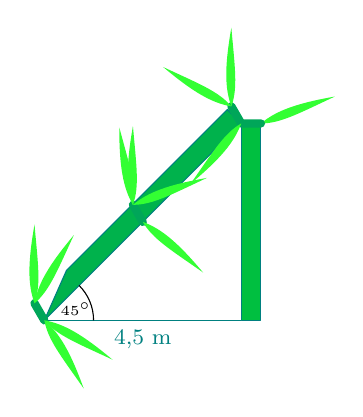
\begin{tikzpicture}[font=\footnotesize, line join=round, line cap=round, >=stealth,scale=0.5]
	%	\pagecolor{yellow!20}
	\tikzset{la/.pic={
	\fill[green!80!white](0,0)..controls++(-20:0.5) and ++(-175:1)..(2,0)..controls++(170:1) and ++(20:0.5)..(0,0);
	}}
	\def\cao{5}
	\def\a{0.1*\cao}
	\pgfmathsetmacro{\dai}{\cao*1}
	\draw[fill=green!75!blue,draw=teal](0,0)rectangle(\a,\cao)pic[rotate=20,scale=0.5]{la};
	\draw[fill=green!70!blue,draw=teal](-\dai,0)--(0,\cao)coordinate(cao)--([turn]90:\a)--([turn]90:{2/sqrt(3)*\dai})--cycle;;
	\draw[teal](-\dai,0)coordinate(dai)--(0,0)coordinate(oo);
	\begin{scope}
	\clip(oo)--(cao)--(dai)--cycle;
	\draw(dai)circle(1.25)++(20:0.85)node{\tiny $45^\circ$};
	\end{scope}
	\draw[line width=3pt,green!65!blue](0,\cao)pic[rotate=-130,scale=0.5]{la}--(\a,\cao)(cao)--++(120:\a)pic[rotate=150,scale=0.5]{la}pic[rotate=90,scale=0.5]{la}(dai)--++(120:\a)(-0.5*\dai,0.5*\cao)pic[rotate=-40,scale=0.5]{la}--++(120:\a)pic[rotate=90,scale=0.5]{la}pic[rotate=20,scale=0.5]{la}pic[rotate=100,scale=0.5]{la};
	\path(dai)pic[rotate=-30,scale=0.5]{la}(dai)pic[rotate=-60,scale=0.5]{la}(dai)++(120:\a)pic[rotate=60,scale=0.5]{la}pic[rotate=90,scale=0.5]{la};
	\path(dai)--(oo)node[pos=0.5,below, teal]{$4{,}5$ m};
	\end{tikzpicture}
	}
	\loigiai{
	\immini{
	Xem đoạn bị gãy là $CB$; đoạn còn lại (thẳng đứng) là $AC$. \\
	Như vậy, độ dài của cây khi chưa bị gãy là $AC+BC$. \\
	Do $\triangle ABC$ vuông tại $A$ và $\widehat{ABC}=45^\circ$, suy ra $\triangle ABC$ vuông cân tại $A$. \\
	Suy ra $AC=AB=4{,}5\mathrm{~m}$. \\
	Áp dụng định lí Pytagore trong $\triangle ABC$ vuông tại $A$, ta được
	$$BC^2=AB^2+AC^2\Rightarrow BC=\sqrt{2\cdot (4{,}5)^2}=\sqrt{40{,}5}\mathrm{~m}.$$
	Chiều cao cây trước khi gãy là $4{,}5+\sqrt{40{,}5}\approx 10{,}9\mathrm{~m}$.
	}
	{
	\begin{tikzpicture}[scale=1,line join=roun,line cap=round,font=\footnotesize,>=stealth]
	\path (0,0) coordinate (A) (0:3) coordinate (B) (90:3) coordinate (C);
	\draw pic[draw, angle radius=3mm]{angle=C--B--A};
	\draw pic[draw, angle radius=2mm]{right angle=C--A--B};
	\draw (A)--(B)--(C)--cycle
	(B)node[shift={(160:.6)},scale=.8]{$45^\circ$}
	;
	\foreach \a/\b in {A/200,B/-30,C/70}{
	\fill[black] (\a)circle(.7pt) ($(\a)+(\b:2mm)$)node[scale=.8]{$\a$};
	}
	\end{tikzpicture}
	}
	}
\end{bt}
%%==========Bài 38
\begin{bt}
	Có hai xã $A$, $B$ cùng ở bên bờ sông Lam, khoảng cách từ hai xã đó đến bờ sông lần lượt là $AA'=500$ m, $BB'=600$ m và người ta đo được $A'B'=2200$ m. Các kĩ sư muốn xây một trạm cung cấp nước sạch nằm bên bờ sông Lam cho người dân hai xã. Giả sử vị trí của trạm cung cấp nước sạch đó là điểm $M$ trên đoạn $A'B'$ với $MA'=x$ (m), $0<x<2200$ (minh họa ở hình bên).
	\begin{center}
	\begin{tikzpicture}[>=stealth,scale=1, line join = round, line cap = round]
	\path (-3,0) coordinate (A')
	(0,0) coordinate (M)
	(4,0) coordinate (B')
	($(A')+(0,2)$) coordinate (A)
	($(B')+(0,3)$) coordinate (B)
	;
	\draw (-5,0)--(A') (A')--(M) node[midway,above]{$x$ (m)} (M)--(5,0);
	\draw (M)--(A) (A)--(A') node[midway,left]{$500$ m} (M)--(B) (B)--(B') node[midway,right]{$600$ m};
	\draw[dashed] ($(A')+(0,-1)$)--(A') ($(B')+(0,-1)$)--(B');
	\draw [<->] ($(A')+(0,-0.8)$)--($(B')+(0,-0.8)$)node[midway,above]{$2200$ m};
	\foreach \x/\goc in {A'/-120,B'/-60,M/90,A/90,B/90}\fill[black]
	(\x) circle (1pt)
	($(\x)+(\goc:3mm)$)node{$\x$};
	\end{tikzpicture}
	\end{center}
	\begin{listEX}[1]
	\item Hãy tính tổng khoảng cách $MA+MB$ theo $x$.
	\item Tính tổng khoảng cách $MA+MB$ khi $x=1200$ (làm tròn kết quả đến hàng đơn vị của mét).
	\end{listEX}
	\loigiai{
	\begin{listEX}[1]
	\item Xét $\triangle AA'M$ vuông tại $A'$ có $MA=\sqrt{AA'^2+A'M^2}=\sqrt{500^2+x^2}$ (m).\\
	Xét $\triangle BB'M$ vuông tại $B'$ có $MB=\sqrt{BB'^2+B'M^2}=\sqrt{600^2+(2200-x)^2}$ (m).\\
	Khi đó $MA+MB=\sqrt{500^2+x^2}+\sqrt{600^2+(2200-x)^2}$ (m).
	\item Khi $x=1200$, ta có $$MA+MB=\sqrt{500^2+1200^2}+\sqrt{600^2+(2200-1200)^2}\approx 2466 \text{ (m)}$$
	\end{listEX}
	}
\end{bt}
%%==========Bài 39
\begin{bt}
	\immini{
	Trên cần trục ở Hình $5$ , hai trụ $a$ và $b$ đứng cách nhau $20$ m, hai xà ngang $c$ và $\mathrm{d}$ lần lượt có độ cao $20$ m và $45$ m so với mặt đất. Xà chéo $x$ có độ dài bao nhiêu mét (kêt quả làm tròn đến hàng đơn vị)?	
	}
	{
	\begin{tikzpicture}[scale=0.75, font=\footnotesize, line join=round, line cap=round, >=stealth]
	\def\canh{6}
	\coordinate (B) at (\canh,3);
	\coordinate (C) at (\canh,0);
	\coordinate (A) at (0,0);
	\coordinate (D) at ($(B)+(A)-(C)$);
	\coordinate (X) at ($(A)!1/5!(C)$);
	\coordinate (Y) at ($(A)!2/5!(C)$);
	\coordinate (Z) at ($(D)!1/5!(B)$);
	\coordinate (Z1) at ($(D)!3/5!(B)$);
	\coordinate (T) at ($(D)!2/5!(B)$);
	\coordinate (X1) at ($(X)!2/5!(Z)$);
	\coordinate (Y1) at ($(Y)!2/5!(T)$);
	\coordinate (T1) at ($(Y)!8/5!(T)$);
	\coordinate (T2) at ($(Y)!1.1!(T)$);
	\coordinate (Z2) at ($(X)!1.1!(Z)$);
	\coordinate (D1) at ($(D)!3/5!(T1)$);
	\draw [line width=0.4mm](A)--(C) (T1)--(B)--(D)--(T1) (X)--(Z2)(Y)--(T) (X1)--(Y1) (X1)--(T)--(T1)--(Z1)
	(D1)--(Z2)--(T2)--(D1)
	;
	\node[below] at ($($(X)+(0,-0.25)$)!0.5!($(Y)+(0,-0.25)$)$){$20\mathrm{~m}$};
	\draw[<->] ($(X)+(0,-0.2)$)--($(Y)+(0,-0.2)$);
	\node[below] at ($($(X1)+(0,-0.05)$)!0.5!($(Y1)+(0,-0.05)$)$){$c$};
	\node[left=0.1cm] at ($($(X)$)!0.5!($(X1)$)$){$20\mathrm{~m}$};
	\draw[<->] ($(X)+(-0.2,0)$)--($(X1)+(-0.2,0)$);
	\node[left=0.1cm] at ($($(X)$)!0.5!($(Z)$)$){$a$};
	\node[right=0.1cm] at ($($(Y)$)!0.5!($(T)$)$){$b$};
	\node[right] at ($($(X1)$)!0.4!($(T)$)$){$x$};
	%\node[above=0.25cm] at ($($(x)+(0,-0.25)$)!0.5!($(B)+(0,-0.25)$)$){$\sqrt{2}\mathrm{~cm}$};
	%\draw[<->] ($(x)+(0,0.2)$)--($(B)+(0,0.2)$);
	\node[right=1cm] at ($($(T)$)!0.5!($(Y)$)$){$45\mathrm{~m}$};
	\draw[<->] ($(T)+(1.3,0)$)--($(Y)+(1.3,0)$);
	\node[below=0.5cm] at ($($(A)+(0,-0.25)$)!0.5!($(C)+(0,-0.25)$)$){Hình $5$};
	\end{tikzpicture}
	}
	\loigiai{
	Theo định lý Pytago ta có $x=\sqrt{c^2+b^2}$.\\
	Theo đề ta có $b=45-20=25$ và $c=20$.\\
	Suy ra $x=\sqrt{25^2+20^2}=\sqrt{1025}\approx32$.\\
	Vậy xà chéo $x$ có độ dài khoảng $32$ m.
	}
\end{bt}
%%==========Bài 40
\begin{bt}
	Hệ quả của hiện tượng nóng lên toàn cầu là băng của một số sông băng đang tan chảy. Mười hai năm sau khi băng biến mất, những loài thực vật nhỏ bé, được gọi là địa y, bắt đầu mọc trên đá. Mỗi nhóm địa y phát triển ở dạng (gần như) một hình tròn. Đường kính $d$ (mm) của hình tròn này và tuổi của địa y có thể được tính gần đúng bằng công thức $d=7\sqrt{t-12}$ với $t$ là số năm tính từ khi băng biến mất ($t \ge 12$) (nguồn: J.Libby, Math for Real Life: Teaching and Practical Uses for Algebra, McFarland, năm 2017). Tính đường kính của hình tròn do địa y tạo nên sau khi băng biến mất $13$ năm; $16$ năm.
	\loigiai{
	Đường kính của hình tròn do địa y tạo nên sau khi băng biến mất $13$ năm \[7\sqrt{13-12}=7 \text{ (mm)}.\]
	Đường kính của hình tròn do địa y tạo nên sau khi băng biến mất $16$ năm \[7\sqrt{16-12}=14 \text{ (mm)}.\]
	}
\end{bt}